%\chapter{Database character study}
\section{Database character study}
\label{sect:db_character_study}
This is just a look at snapshots of the deployed ODB and various generated datasets to determine general characteristics and limits. A useful test is to examine the contention profile generated by various models by perfoming an overnight simulation - this differs from the prior contention profile which does not take into account those observations performed earlier in the night.

A set of standard execution models was generated:-these belong in 

\begin{table}[h]
\begin{center}
\begin{tabular}{lllllll}
\toprule
\multicolumn{5}{c}{Standard Execution Timing Models} \\
\midrule
Name & Offset(s) & Readout(s) & Slew(s) & Config(s) & MaxT(H) & Horizon($^{\circ}$) \\
\midrule
$X_{n/S}$      & 10     & 12      & 60   & 6  &  2  & 20 \\
$X_{n/L}$      & 10     & 12      & 60   & 6  &  4  & 20 \\
$X_{n/L/hi}$   & 10     & 12      & 60   & 6  &  4  & 30 \\
$X_{f/S}$      & 5      & 6       & 45   & 4  &  2  & 20 \\
$X_{f/L}$      & 5      & 6       & 45   & 4  &  4  & 20 \\
$X_{f/L/hi}$   & 5      & 6       & 45   & 4  &  4  & 30 \\
$X_{s/S}$      & 12     & 16      & 90   & 12 &  2  & 20 \\ 
$X_{s/L}$      & 12     & 16      & 90   & 12 &  4  & 20 \\ 
$X_{s/L/hi}$   & 12     & 16      & 90   & 12 &  4  & 30 \\ 
\bottomrule
\end{tabular}
\end{center}
\caption{Set of standard execution models. Classified as \emph{slow} (s), \emph{normal} (n) and \emph{fast} (f), with maximum execution times \emph{short} (S) and \emph{long} (L). \emph{Hi} models have extra high horizon. Additional models defined based on these but with e.g. MaxT 30 minutes and horizon elevation 35$^{\circ}$ would be specified as $X_{n/30m/35d}$. }
\end{table}

Description of various characterisation simulations.
\begin{itemize}
\item demand profiles/load stats (all available snapshot nights using DC and LC.) -- dont diplay all these as latex will thorw a wobbly, jsut a selection for now.
\item Demand and load averages and min/max plot over whole season along with nightlength, moondark/astronight plots. Figure \ref{fig:cd_av_trend} shows the trend of $C_D$ over the available set of ODB snapshots.


\item run BST for a selection of nights multiple times to get contention (ensemble) plots over nights under efx,efp and several e-scenarios (make sure these are tabulated seperately).
\end{itemize}

% CD trend and max plots
\begin{figure}[h]
\begin{center}
 \subfigure[Trend of average value of demand profile $C_D$ for available ODB dataset]{
   \includegraphics[scale=0.5, angle=-90]{figures/cdtrend.eps}
   \label{fig:cd_av_trend}
 }

 \subfigure[Trend of peak value of demand profile $C_D$ for available ODB dataset]{
   \includegraphics[scale=0.5, angle=-90]{figures/cdmax.eps}
   \label{fig:cd_max_trend}
 }
\caption{Trends of demand statistics over available ODB snapshots}
\end{center}
\end{figure}

%CL trend plots
\clearpage
\begin{figure}[h]
\begin{center}
 \subfigure[Trend of nightly number of groups executed for available ODB dataset]{
   \includegraphics[scale=0.25, angle=-90]{figures/cl_ngs.eps}
   \label{fig:db_cl_ngs}
 }
 \subfigure[Trend of nightly load $C_L$ and $C_{CL}$ for available ODB dataset]{
   \includegraphics[scale=0.25, angle=-90]{figures/cl_load.eps}
   \label{fig:db_cl_load}
 }
 \subfigure[Trend of nightly weighted load $C_{PL}$ and $C_{UL}$ for available ODB dataset]{
   \includegraphics[scale=0.25, angle=-90]{figures/cl_puload.eps}
   \label{fig:db_cl_puload}
 }
\caption{Trends of load statistics over available ODB snapshots}
\end{center}
\end{figure}


\subsection{Experiments}
Notes about some experiments to do (these dont belong here)

\begin{enumerate}

\item Calculate total schedulable time in a night and advance demand profiles.

Search p2db for any groups which are enabled that night and sum up total exec times. If they are monitors we need to add n times exec (for n windows). If flexible we should count seperately or maybe add in a fractional contribution for 1/(length (nights) of flex span). Similar for ephem groups. Do this for a year or semester - note the flex stuff becomes a bit weird as some would have been done do we want to deplete them as if actually done (P(done before tonight) = (t-flexstart)/span or the likes). want to normalize results by length of night (sus-sur or twi-twi). As weel as semesterly would be good to get this information as a profile for individual nights and showing subscription(t), priority(t) etc.

This is an indicator of over/under subscription. If we are undersubscribed any night we should be able to accomodate everything with a bit of negotiation /sliding. If oversubscribed then need to prioritize - e.g. auction prices set by demand ! The oversubscription rate is a useful piece of info to give PDAs - lets them know how bad competition is without divulging sensitive information from other PDAs. Also could allow view of profiles over the night of PDA requests by priority level. 

Scenario: start of night, SE asks PDAs to make reservations (not really just what i would like to get and what priority or \emph{score} is assigned  - by PDA or normallized? - no commitment but expect truthful!). SE makes profiles available to all PDAs. This sort of thing would let a PDA see if there were quiet or low priority slots available again without divulging too much information - any sort of statistical info like this is potentialy useful in decision making for bidding. 


\item Monte-carlo simulation to find range of scores using simple scheduling algorithm(s).

Step thro night, pick a group from feasibles (random selection), if none timestep a minute or so else time step exec time, repeat.
Count up total used time. count sum priorities, count cumulative score via various metrics.

Repeat this umpteen times to get ranges, mean and stds for these parameters and measuring score metrics using various parameterisations.

Want to see the range of schedules we could get to set some bounds on these. We would expect a real scheduler to do better than the worst case and hopefully as good as best case. We wont see the best case unless we do zillions of runs but may get some idea how far into the tail it is..

\item Various contention measures

\begin{itemize}
\item True contention over night as profile
\item Daily groups enabled in night at some point count over period of weeks/months
\item Daily groups enabled over night as profile
\item weighted contention profile
\item Probabilistic true contention as profile over night with different seeing assumptions -i.e. different curves and then various probabilty assumption curves plus a combined probabilty curve, maybe some envelopes.
\end{itemize}


\item Some notes about the simulation framework.

\end{enumerate}
